\documentclass[12pt]{article}

\usepackage[a4paper,margin=1in]{geometry}
\usepackage{amsmath,amssymb}
\usepackage{graphicx}
\usepackage{tikz}
\usepackage[none]{hyphenat}

\setlength{\parindent}{0pt}
\setlength{\parskip}{6pt}

\begin{document}

%================ HEADER =================%

\begin{enumerate}
\item[] \centering
\includegraphics[width=4.5cm]{iiitb_logo.png}

\item[] \centering
\textbf{Keshava Reddy V}

\item[] \centering
\textbf{ID: COMETFWC054}

\item[] \centering
\textbf{45th IMO 2004}
\end{enumerate}

\vspace{0.6cm}

%================ PROBLEMS =================%

\begin{enumerate}

\item \textbf{Problem 1.}
Let $ABC$ be an acute-angled triangle with $AB \ne AC$.
The circle with diameter $BC$ intersects the sides $AB$ and $AC$ at $M$ and $N$
respectively. Denote by $O$ the midpoint of the side $BC$.
The bisectors of the angles $\angle BAC$ and $\angle MON$ intersect at $R$.
Prove that the circumcircles of the triangles $BMR$ and $CNR$
have a common point lying on the side $BC$.

\item \textbf{Problem 2.}
Find all polynomials $f$ with real coefficients such that for all real numbers
$a,b,c$ satisfying $ab + bc + ca = 0$ we have
\[
f(a-b) + f(b-c) + f(c-a) = 2f(a+b+c).
\]

\item \textbf{Problem 3.}
Define a ``hook'' to be a figure made up of six unit squares as shown below,
or any of the figures obtained by applying rotations and reflections to this figure.

\begin{enumerate}
\item[] \centering
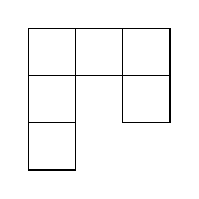
\begin{tikzpicture}[scale=0.6]
\draw (0,2) rectangle (1,3);
\draw (1,2) rectangle (2,3);
\draw (2,2) rectangle (3,3);
\draw (0,1) rectangle (1,2);
\draw (0,0) rectangle (1,1);
\draw (2,1) rectangle (3,2);
\end{tikzpicture}
\end{enumerate}

Determine all $m \times n$ rectangles that can be covered without gaps and without overlaps
with hooks such that
\begin{itemize}
\item the rectangle is covered without gaps and without overlaps;
\item no part of a hook covers area outside the rectangle.
\end{itemize}

\item \textbf{Problem 4.}
Let $n \ge 3$ be an integer.
Let $t_1,t_2,\ldots,t_n$ be positive real numbers such that
\[
n^2 + 1 >
(t_1 + t_2 + \cdots + t_n)
\left(
\frac{1}{t_1} + \frac{1}{t_2} + \cdots + \frac{1}{t_n}
\right).
\]
Show that $t_i,t_j,t_k$ are side lengths of a triangle for all
$1 \le i < j < k \le n$.

\item \textbf{Problem 5.}
In a convex quadrilateral $ABCD$ the diagonal $BD$ does not bisect the angles
$\angle ABC$ and $\angle CDA$.
The point $P$ lies inside $ABCD$ and satisfies
\[
\angle PBC = \angle DBA
\quad \text{and} \quad
\angle PDC = \angle BDA.
\]
Prove that $ABCD$ is a cyclic quadrilateral if and only if $AP = CP$.

\item \textbf{Problem 6.}
We call a positive integer alternating if every two consecutive digits in its
decimal representation are of different parity.
Find all positive integers $n$ such that $n$ has a multiple which is alternating.

\end{enumerate}

\vfill
\begin{enumerate}
\item[] \centering 1
\end{enumerate}

\end{document}



